\chapter{Métrica mixta}
En este capítulo utilizaremos los resultados obtenidos en el capítulo anterior para desarrollar una variante al procedimiento córte de árbol dinámico que integre la información contenida en el espacio de expresión con la información contenida en el espacio de conocimientos GO, para favorecer la búsqueda de estructuras biológicamente coherentes. La idea principal de esta variante es la de montar sobre la heterogeneidad topológica (transcripcional) un desorden de pesos a partir de la información biológica, y con ello obtener una métrica mixta que contenga información de ambos espacios.

\section{Hacia una métrica mixta}
Existen muchas formas de mezclar las métricas del espacio de expresión y del espacio GO. Una de las métricas mixtas investigadas previamente por el grupo \cite{Berenstein2010} fue la de mezcla convexa de distancias, donde se define una nueva distancia $d_{mix}$ a partir de las distancias de expresión y GO y un parámetro $\alpha$ que controla la contribución de cada métrica al algoritmo:
\begin{equation}
	d_{mix} = \sqrt{\alpha d_{x}^2 + (1-\alpha)\tilde{d}_{GO}^2}
\end{equation}
con $\tilde{d}_{GO} = \frac{\langle d_x \rangle}{\langle d_{GO} \rangle}d{_GO}$, de tal manera que coincidan los valores medios de ambas distribuciones de distancia.\\
Esta métrica busca el consenso a partir del parámetro global $\alpha$, que parametriza de manera continua una métrica en contraposición con la otra.\\
Para este trabajo, implementamos una métrica mixta que en lugar de buscar el consenso entre las métricas, penaliza las correlaciones no soportadas por las distintas ontologías e incentiva aquellas que si lo están .
\subsection{Modificación de la similaridad de correlación}
Para obtener una métrica que permita detectar heterogeneidades dentro de los grupos, modificamos la similaridad de correlación utilizando la información obtenida mediante el índice KTA local en las redes de 30 primeros vecinos mutuos.\\
Para ello, tomamos cada grupo de cada tratamiento y calculamos el KTA de todo el grupo, además del KTA local de cada arista del grupo. Estas dos cantidades, el KTA de grupo, que llamaremos $KTA_{fondo}$, y el KTA local de la arista entre dos nodos $i$ y $j$, que llamaremos $KTAl_{ij}$, se relacionan en una cantidad llamada $stress$ que utilizaremos como criterio para identificar si debemos penalizar o incentivar una correlación en el espacio de expresión. El $stress$ se define como:
\begin{equation}
	stress = \frac{KTA_{fondo}}{KTAl_{ij}}
\end{equation}
Si $KTAl_{ij} > KTA_{fondo}$, se obtiene un $stress < 1$, mientras que si $KTAl_{ij} < KTA_{fondo}$, obtenemos que $strees > 1$. Por lo tanto, si realizamos la transformación no lineal de la similaridad de correlación:
\begin{equation}
	w_{ij} = simcor_{ij}^{stress}
	\label{eq:stress}
\end{equation}
obtenemos unos nuevos pesos para la similaridad de correlación en donde aquellas relaciones que son similares en GO ($KTAl_{ij} > KTA_{fondo}$) serán incentivadas en el espacio de expresión y a la inversa, las que no son similares en GO serán penalizadas en el espacio de expresión. La figura \ref{fig:distribucion_de_stress} presenta la distribución de $stress$ para el tratamiento 'Frío' en función del tamaño de grupo. Se observa que el $92\%$ de los valores de $stress$ se ubica entre $0.8$ y $1.2$. 
\begin{figure}[H]
\centering
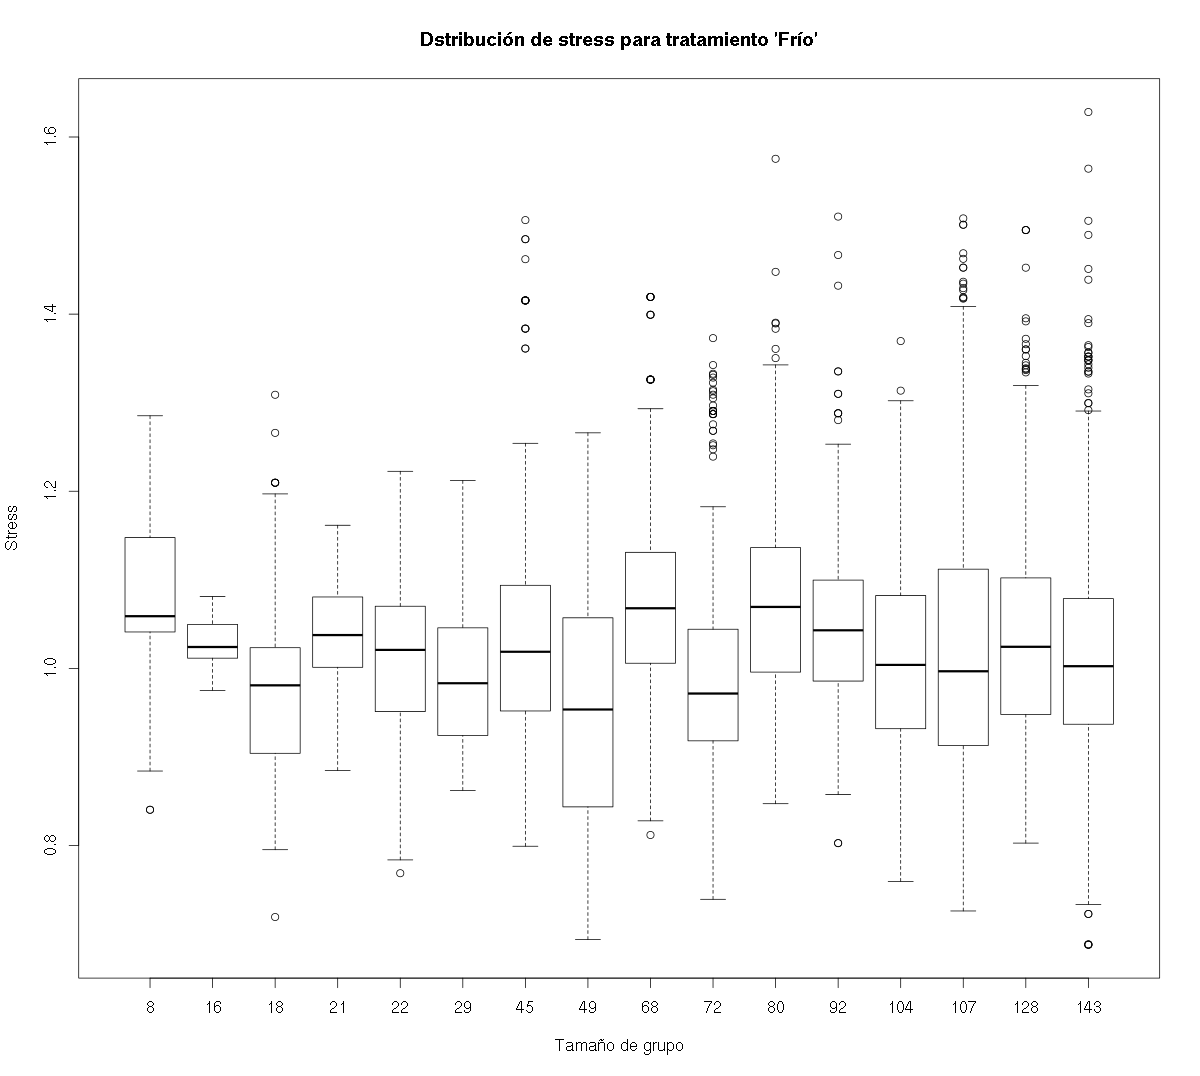
\includegraphics[height=0.8\textwidth]{distribucion_de_stress}
\caption{Distribución de $stress$ para el tratamiento 'Frío' y ontología CC en función del tamaño de grupo.}
\label{fig:distribucion_de_stress}
\end{figure}
Este rango en los valores del $strees$ no permite penalizar adecuadamente las similaridades en el espacio de expresión, lo que implica que será necesario modificar la escala del $strees$ proporcionalmente por medio de un parámetro $\beta$, de tal forma que los pesos de la ecuación \ref{eq:stress} se transformen como:
\begin{equation}
	\tilde{w_{ij}} = w_{ij}^{\beta}
	\label{eq:pesos_beta}
\end{equation}
Para encontrar el beta adecuado, haremos uso de la información contenida en la red.\\
Como analizamos en el capítulo anterior, las redes de k primeros vecinos mutuos no poseen una distribución de grado con cola pesada. Una cola pesada es indicativo de que la distribución de grado sigue una ley de potencias, es decir, $p(k) \approx k^{-\gamma}$, y por lo tanto la red tiene una topología de tipo libre de escala. Muchas redes reales son de este tipo.\\
Horvath, en \cite{Horvath2005}, propone buscar un parámetro $\beta$ al cual elevar la similaridad de correlación de genes tal que la red de genes obtenida siga una distribución de tipo ley de potencias.\\
Buscamos el parametro $\beta$ adecuado realizando un barrido para $\beta$ desde 1 hasta 4 con pasos de 1 y desde 15 hasta 65 con pasos de 5, transformando los pesos de la red $w_{ij}$ mediante la ecuación \ref{eq:pesos_beta} y realizando un ajuste lineal para el logaritmo de los pesos en función del logaritmo de la probabilidad. Tomamos el parámetro $\beta$ que mejor ajustaba cada tratamiento en el sentido de R cuadrado y lo utilizamos para modificar los pesos $w_{ij}$. Por ejemplo, para el tratamiento 'Frío', obtuvimos $\beta=4$, mientras que para 'Calor' obtuvimos $\beta=55$.
Una vez obtenidos los parámetros para la métrica mixta, desarrollamos un método heurístico para poder aplicar esta nueva métrica mixta.
\section{Método heurístico}
El método heurístico desarrollado consiste en tomar cada grupo de una partición realizada previamente con corte de árbol dinámico e intentar particionarlo de tres formas distintas.\\
La primera forma consiste en aplicar sobre cada grupo nuevamente corte de árbol dinámico, utilizando la métrica mixta en la confección del dendrograma, penalizando (incentivando) las conexiones más importantes, que son las que aparecen en la red de k primeros vecinos mutuas con alto (bajo) stress, método que llamaremos \textit{lkta.dtc}. Por otro lado, la segunda y la tercera formas, que llamaremos \textit{lkta.infomap} y \textit{lkta.cnm}, consisten en obtener comunidades mediante infomap y cnm, respectivamente, en la red de los genes del grupo con los pesos modificados por la métrica mixta. Una vez obtenida una partición del grupo, calculamos el índice BHI de los subgrupos y volvemos a unir aquellos subgrupos que se encuentren por debajo de una desviación estandar del control nulo 1 presentado en la sección \ref{subsec:control_nulo} mediante un algoritmo voraz o greedy, que en cada paso busca los dos subgrupos tales que el BHI de los dos juntos sea superior al BHI de cada uno por separado. Cuando el algoritmo no consigue unir dos subgrupos para mejorar el BHI, se detiene.\\ Finalmente, todos los subgrupos que todavía quedan por debajo de una desviación estandar del control nulo 1 son unidos entre sí en un único subgrupo.\\
Utilizaremos un cuarto método, llamado \textit{insideX}, a modo de control. El mismo consiste en volver a particionar cada grupo usando corte de árbol dinámico, pero sin cambiar la métrica por la métrica mixta. Esto nos permitirá controlar la efectividad de la métrica mixta para encontrar mayor resolución en las particiones.\\
Para cuantificar el cambio en la información biológica que brinda la nueva partición, elegimos tomar el valor medio del BHI de los subgrupos en comparación con el BHI del grupo original, $\langle BHI \rangle$, y el valor medio del BHI de los subgrupos que superan el control nulo, $\langle BHI \rangle _{+}$. 
A modo de ejemplo, presentamos en las figuras \ref{fig:metodos_mixtos_grupo_2} y \ref{fig:metodos_mixtos_grupo_9} los resultados de esta heurística aplicada a los grupos 2 y 9 del tratamiento 'Frío'. En las mismas, la curva roja indica el valor medio para la distribución del BHI del control nulo 1, la verde una desviación estandar por sobre la media y la negra, una desviación estandar por debajo. El punto lleno representa el grupo original y su BHI. En verde si su BHI supera el control nulo y en rojo si no. Los puntos vacíos en gris representan los subgrupos nuevos. En la leyenda, el primer número es $\langle BHI \rangle$ y el segundo, entre paréntesis, es $\langle BHI \rangle _{+}$.\\
\begin{figure}[H]
\centering
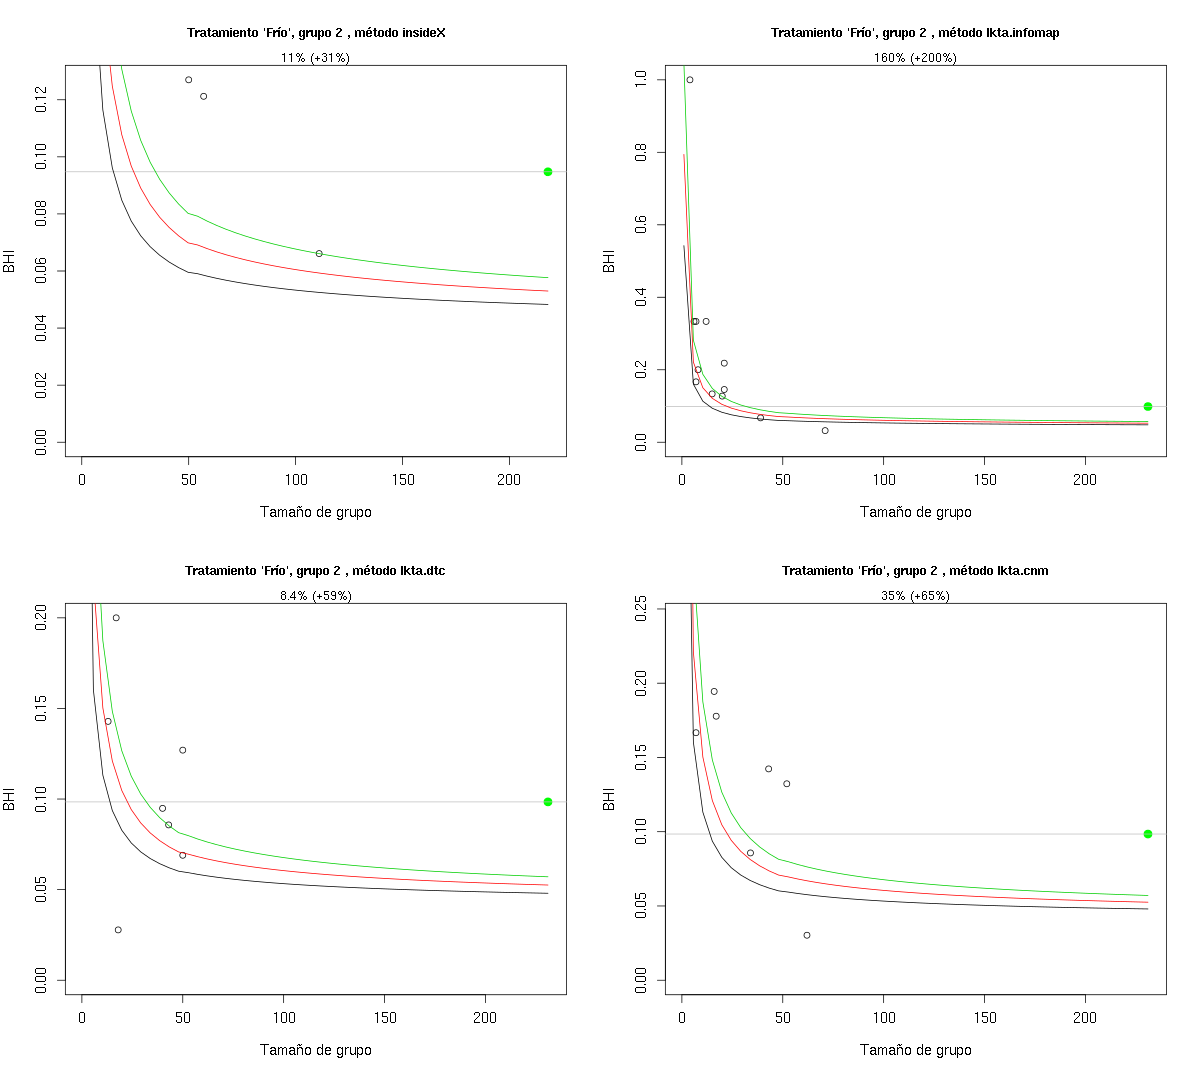
\includegraphics[height=0.8\textwidth]{metodos_mixtos_grupo_2}
\caption{Métodos con métrica mixta y control para el grupo 2 del tratamiento 'Frío'.}
\label{fig:metodos_mixtos_grupo_2}
\end{figure}
\begin{figure}[H]
\centering
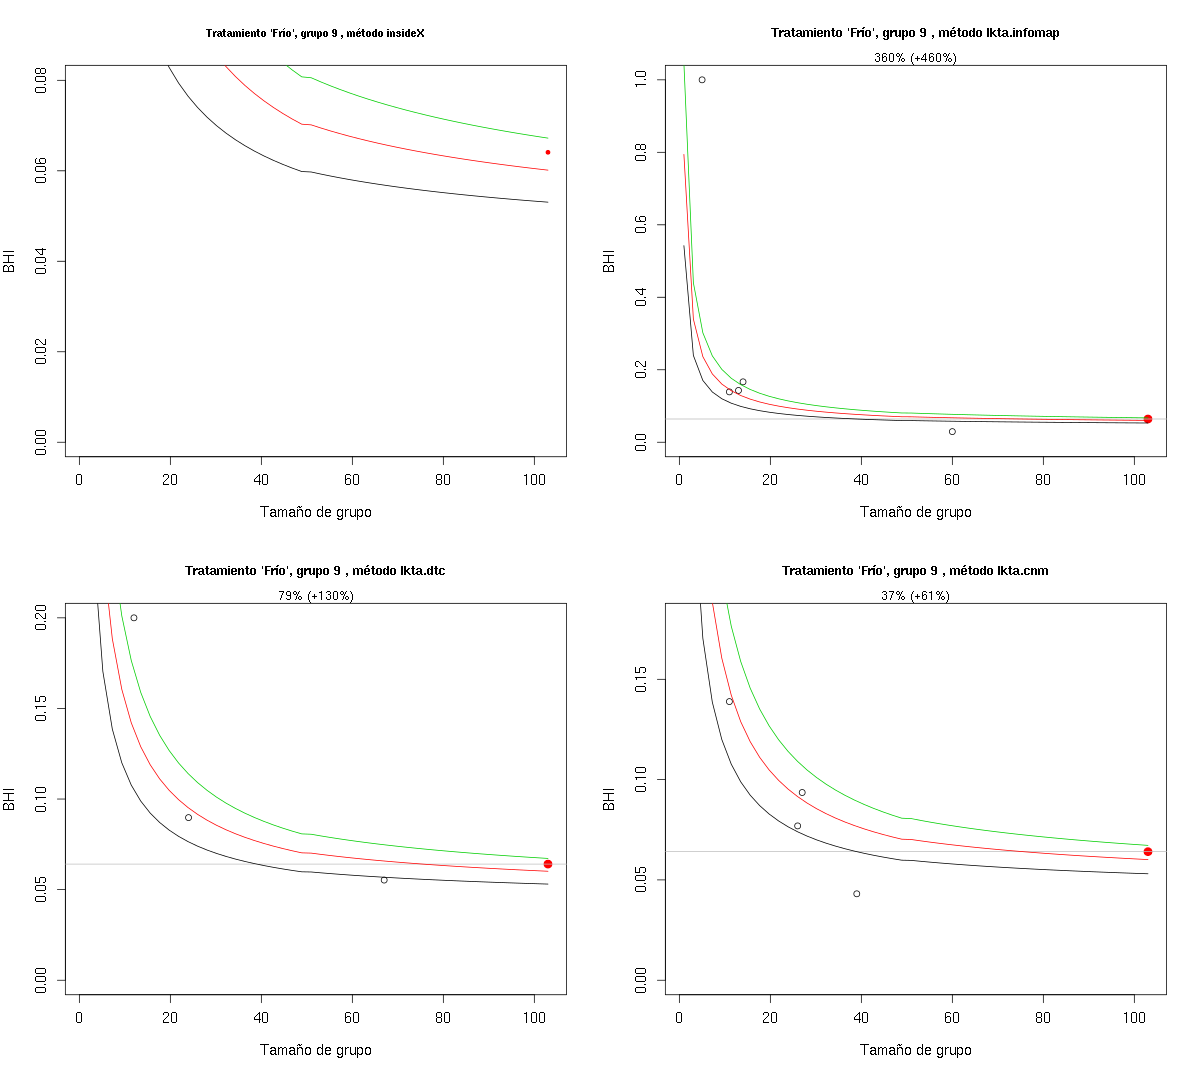
\includegraphics[height=0.8\textwidth]{metodos_mixtos_grupo_9}
\caption{Métodos con métrica mixta y control para el grupo 9 del tratamiento 'Frío'.}
\label{fig:metodos_mixtos_grupo_9}
\end{figure}
Se observa que para el grupo 2, un grupo con un BHI por sobre el control nulo y el segundo grupo más grande de la partición, el método \textit{insideX} logró encontrar heterogeneidades y partir el grupo, obteniendo tres subgrupos de más de 50 genes cada uno y una mejora del 11\% en $\langle BHI \rangle$, y una del 31\% para $\langle BHI \rangle _{+}$. Por otro lado, los tres métodos \textit{lkta} lograron superar la mejora obtenida por \textit{insideX} en $\langle BHI \rangle _{+}$, y tanto \textit{lkta.infomap} como \textit{lkta.cnm} lograron mejorar además el obtenido en $\langle BHI \rangle$, siendo \textit{lkta.infomap} el que mejores puntajes logró, llegando a obtener incluso un grupo con un BHI de $0.97$.\\
Para el grupo 9, un grupo con un BHI por debajo del control nulo y relativamente pequeño, el método \textit{insideX} no logró encontrar heterogeneidades dentro del grupo y por lo tanto no pudo particionarlo, sin lograr ningún tipo de mejora en el mismo. Sin embargo, todos los métodos \textit{lkta} lograron particionar el grupo y mejorar ambos índices, siendo nuevamente \textit{lkta.infomap} el que logró la mejora más significativa, con un 360\% de incremento en $\langle BHI \rangle$ y un 460\% de incremento en $\langle BHI \rangle _{+}$.\\
Finalmente, realizamos este análisis para todos los tratamientos y todos los grupos en cada tratamiento.\hl{hacer este grafico y terminar el capitulo}




